\section{\label{s:hw}Hardware}

\subsection{\label{ss:phMon}Phase Monitors}

\begin{figure}
  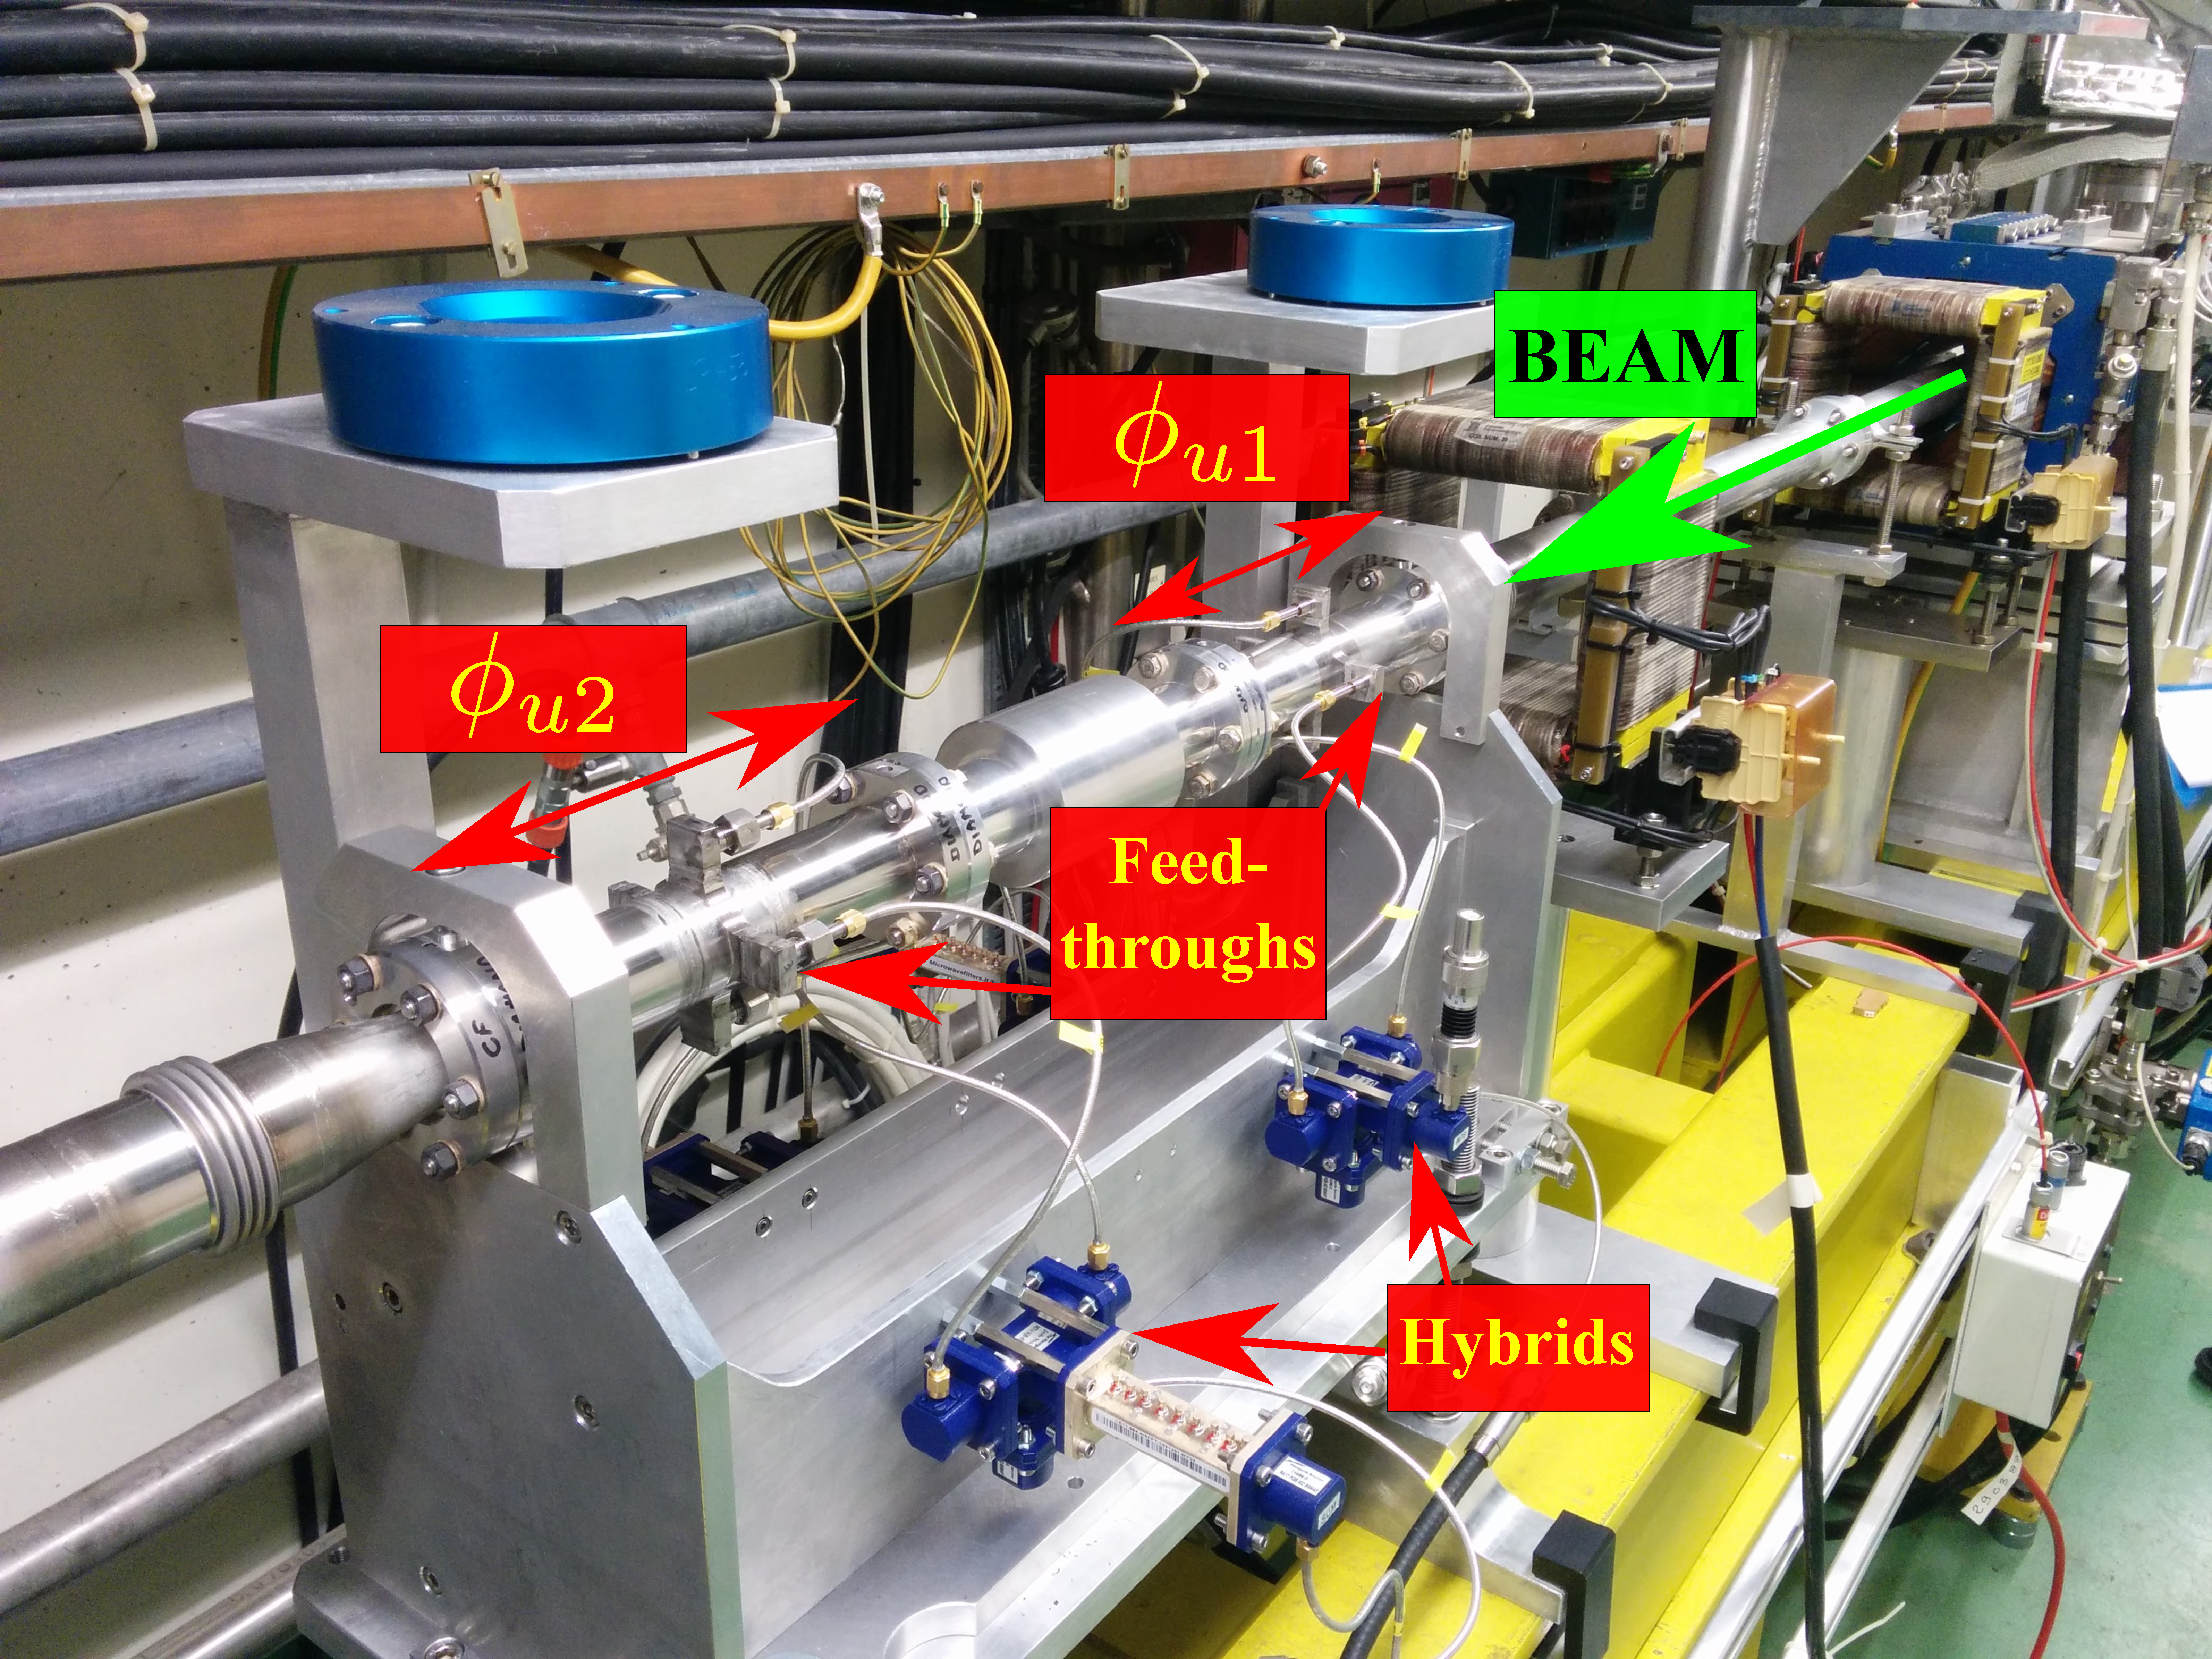
\includegraphics[width=\columnwidth]{phMonCTPic}
  \caption{\label{f:phMonCTPic}The installation of the upstream phase 
    monitors (\(\phi_{u1}\) and \(\phi_{u2}\)) in the beam line.}
\end{figure}

Three phase monitors were installed at CTF3 for the PFF prototype -- two 
neighbouring monitors upstream, \(\phi_{u1}\) and \(\phi_{u2}\), and one 
downstream of the correction chicane, \(\phi_{d}\). Fig.~\ref{f:phMonCTPic} 
shows the installation of the upstream phase monitors 
in the beam line. The upstream monitors are 
used to provide the PFF input (typically \(\phi_{u1}\)), and to measure the 
phase monitor resolution. The notation \(\phi_u\) 
will be used where the distinction between the measurements at \(\phi_{u1}\) 
and \(\phi_{u2}\) is unimportant. The downstream monitor, \(\phi_{d}\), is used 
to measure the effect of the PFF correction.

The phase monitors are cylindrical cavities with an external device length of 
approximately 19~cm and an internal diameter of 23~mm. Small ridges (notch 
filters) in the cavity create 
a volume resonating at 12~GHz (the CLIC drive beam frequency) which contains 
the beam induced fields and reflects any stray 12~GHz fields. The signals are 
extracted through horizontal and vertical pairs of rectangular waveguides, 
before transitioning to 50~\(\mathrm{\Omega}\) coaxial cable via RF 
feedthroughs \cite{phMonIPAC10}. The cavities support the TM01 monopole and 
TE11 dipole modes. The position dependent dipole mode is removed by summing the 
pair of vertical outputs in 180 degree hybrids. The horizontal pair is 
instrumented in the same way but typically is not used. 

\begin{figure}
  \includegraphics[width=\columnwidth]{racks}% Here is 
  %how to 
  %import EPS art
  \caption{\label{f:racks}The two racks containing the PFF system hardware -- 
    the phase monitor electronics, feedforward controller and the kicker 
    amplifiers.}
\end{figure}

The electronics used to extract the phase measurement from the cavity signals 
are installed on the floor above the machine hall in the CTF3 ``klystron 
gallery'', alongside the other hardware used for the PFF system 
(Fig.~\ref{f:racks}). 
Each set of electronics produces two outputs - a phase 
dependent ``mixer'' signal, and a power dependent ``diode'' signal. 

The beam induced signal from the cavities is down-mixed with a 12~GHz local 
oscillator (LO) to create the mixer output. The LO is generated 
from a common 3~GHz source that is phase-locked to the CTF3 drive beam.
Each set of electronics has dedicated frequency multipliers, to increase the LO 
frequency to 12~GHz, and phase shifters, used for calibrations (see below). 
Digital phase shifters originally installed in the system were replaced with 
passive mechanical devices to reduce noise and improve the phase resolution 
[ref].

To be able to operate the mixers at low power (to improve linearity) whilst 
maintaining a large signal to noise ratio (to improve resolution) eight 
separate mixers and diodes are used in each set of electronics \cite{alex09}. 
The inputs are split between the eight mixers and diodes, with the final two 
outputs being the sum of the individual mixer and diode signals. 
Fig.~\ref{f:phMonDiagram} shows a simplified example of this with two 
mixers and diodes. 

\begin{figure}
  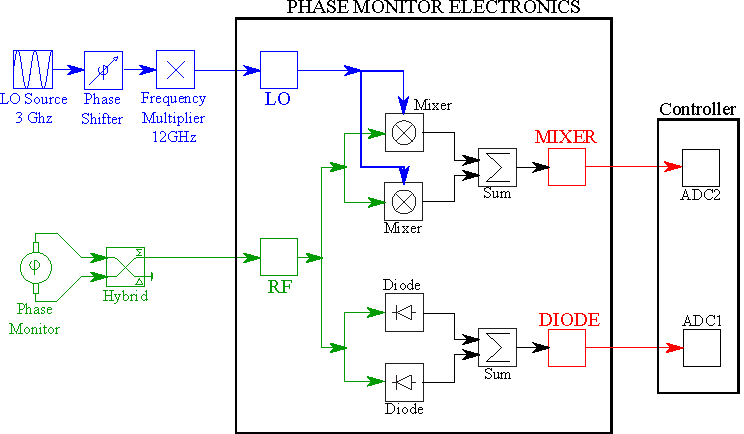
\includegraphics[width=\columnwidth]{phMonDiagram}% Here is 
  %how to 
  %import EPS art
  \caption{\label{f:phMonDiagram}Simplified schematic showing the components 
  involved in the phase calculation. Two individual mixers and diodes are 
  shown in the electronics, compared to eight in the actual design.}
\end{figure}

The diode output was intended to be used to power normalise the mixer output. 
However, an unforeseen design issue with the electronics resulted in the diodes 
saturating at a much lower input voltage than the mixers 
(Fig.~\ref{f:MixDioVsVolts}). To be able to achieve the best possible 
resolution from the mixers, the electronics were operated with the diodes 
saturated, and the diode outputs were not used in the phase reconstruction as 
envisaged. As a consequence, calibrations had to be repeated regularly to 
account for any differences in output power from the cavities resulting from 
changes to the beam setup.

\begin{figure}
 \centering
  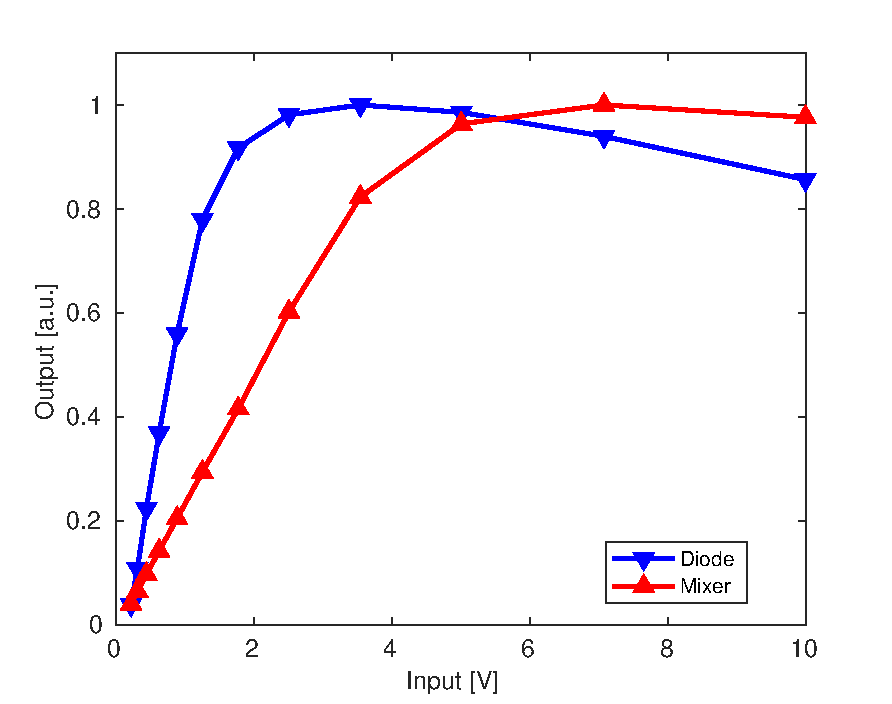
\includegraphics[width=0.6\columnwidth]{MixDioVsVolts}
  \caption{\label{f:MixDioVsVolts}Electronics diode and mixer output 
  amplitudes (normalised with respect to their peak output) versus the input 
  voltage.}
\end{figure}

% FROM THESIS
The phase, \(\phi(t)\), was therefore calculated from the ``Mixer'' outputs as 
follows:
\begin{align}
  &\mathrm{Mixer}(t) = A\sin[\phi(t)] + d \\
  &\phi(t) = \arcsin\left(\frac{\mathrm{Mixer}(t)-d}{A}\right)
  \label{e:phaseRecUsed}
\end{align}
Two calibration constants are needed -- \(A\) and \(d\). \(A\) is the fitted 
(power dependent) 
amplitude of the sinusoidal mixer output, and \(d\) is the asymmetry or offset 
between the maximum and minimum mixer output.
% /FROM THESIS

The calibration constants for each set of electronics are determined by using 
the phase shifters in the LO chains to vary the phase difference between the LO 
input and the beam signal through \(360^\circ\) at 12~GHz. 
Fig.~\ref{f:phMonCal} shows the results of such a calibration. The output from 
the mixers is attenuated to be contained within the \(\pm 
0.5\)~V range of the feedforward controller inputs. The calibration constants 
calculated from the sinusoidal fit to the data points are summarised in 
Table~\ref{t:phMonCal}.

Agreement between data and fit.
 
\begin{figure}
  
  \hfill
  \captionsetup{width=.45\linewidth}%
  \subfloat[][Variation in pulse shape during the 
             calibration. Each line corresponds to a different phase shifter setting at \(\phi_{u1}\).]
   {
    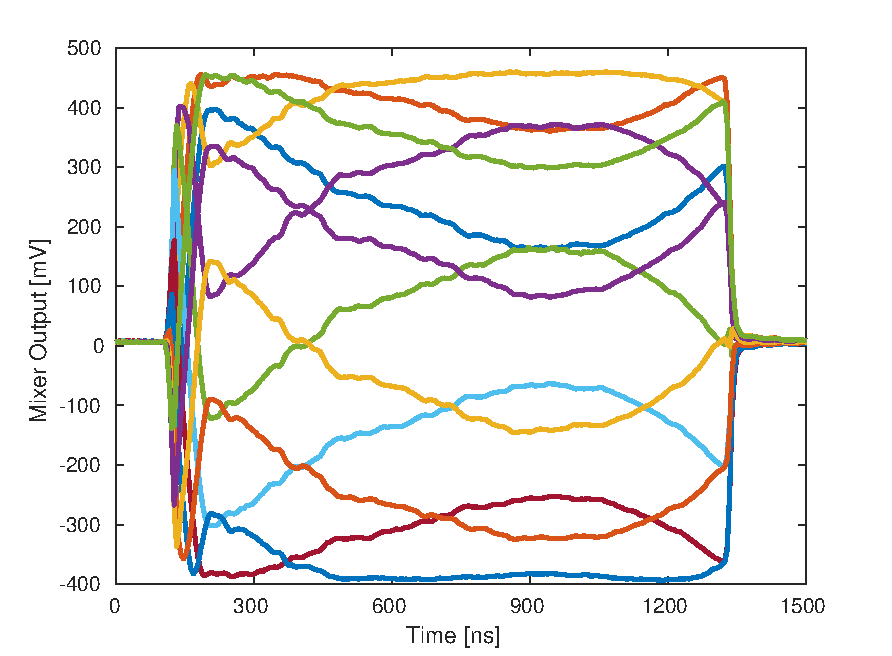
\includegraphics[width=0.47\textwidth]{phMonCalTraces}
    \label{f:calTraces}
   }
  \subfloat[][Response of each mixer output whilst varying 
              the LO phase shifters, at the sample at 933.2~ns in (a). Markers show 
              the measured data points, and lines 
              sinusoidal fits to the data.]
   {
    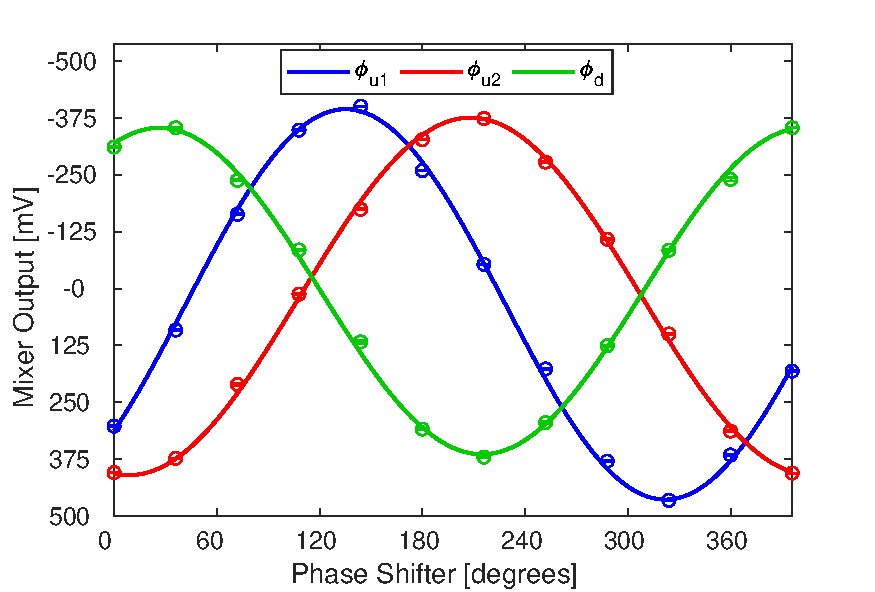
\includegraphics[width=0.515\textwidth]{phMonCal}
    \label{f:loScan}
   }
   
 \centering
 \captionsetup{width=.65\linewidth}%
  \subfloat[][Fitted calibration constants from (b):  \(A\), amplitude, and \(d\), offset.]
   {
      \begin{tabular}{ccc}
        Monitor & \(A\) [mV] & \(d\) [mV] \\
        \hline
        \(\phi_{u1}\) & \(419 \pm 5\) & \(-34 \pm 4\) \\
        \(\phi_{u2}\) & \(383 \pm 2\) & \(-16 \pm 2\) \\
        \(\phi_{d}\) & \(350 \pm 5\) & \(-5 \pm 5\) \\
      \end{tabular}
    \label{t:phMonCal}
    }
  \caption{\label{f:phMonCal}Typical example of the results of a phase   monitor calibration.}
\end{figure}

Zero crossing

Point by point and mean resolution

Bandwidth

Position dependence

% FROM THESIS
Figure~\ref{f:horizontalPosScan} shows the results of a horizontal position 
scan in the upstream phase monitors, with the phase plotted against the 
horizontal position in the BPM.

Taking the calculated position dependence of Mon~1 and Mon~2 this corresponds 
to only an additional measured phase jitter of roughly \(0.04^\circ\), using 
the larger dependence in the horizontal plane. This is small compared to the 
phase monitor resolution
% /FROM THESIS

%\begin{figure}
%  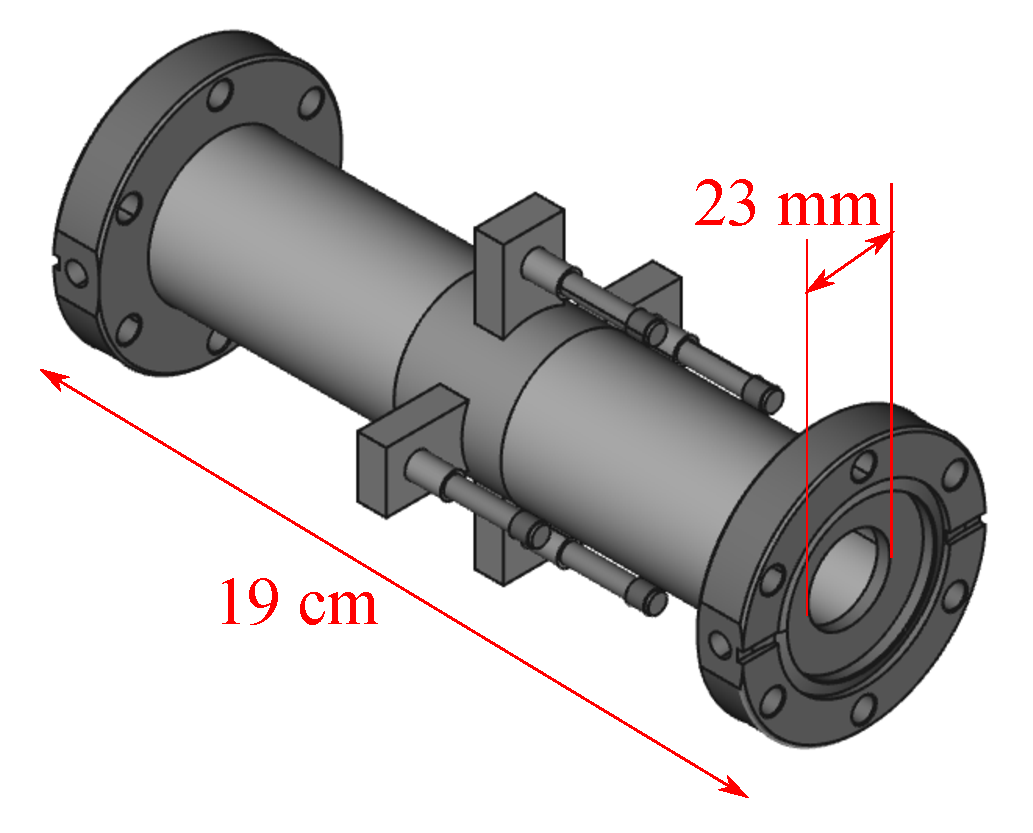
\includegraphics[width=\columnwidth]{phMonTechDraw}% Here is 
%  %how to 
%  %import EPS art
%  \caption{\label{f:phMonTechDraw}
%  }
%\end{figure}
%\begin{figure}
%  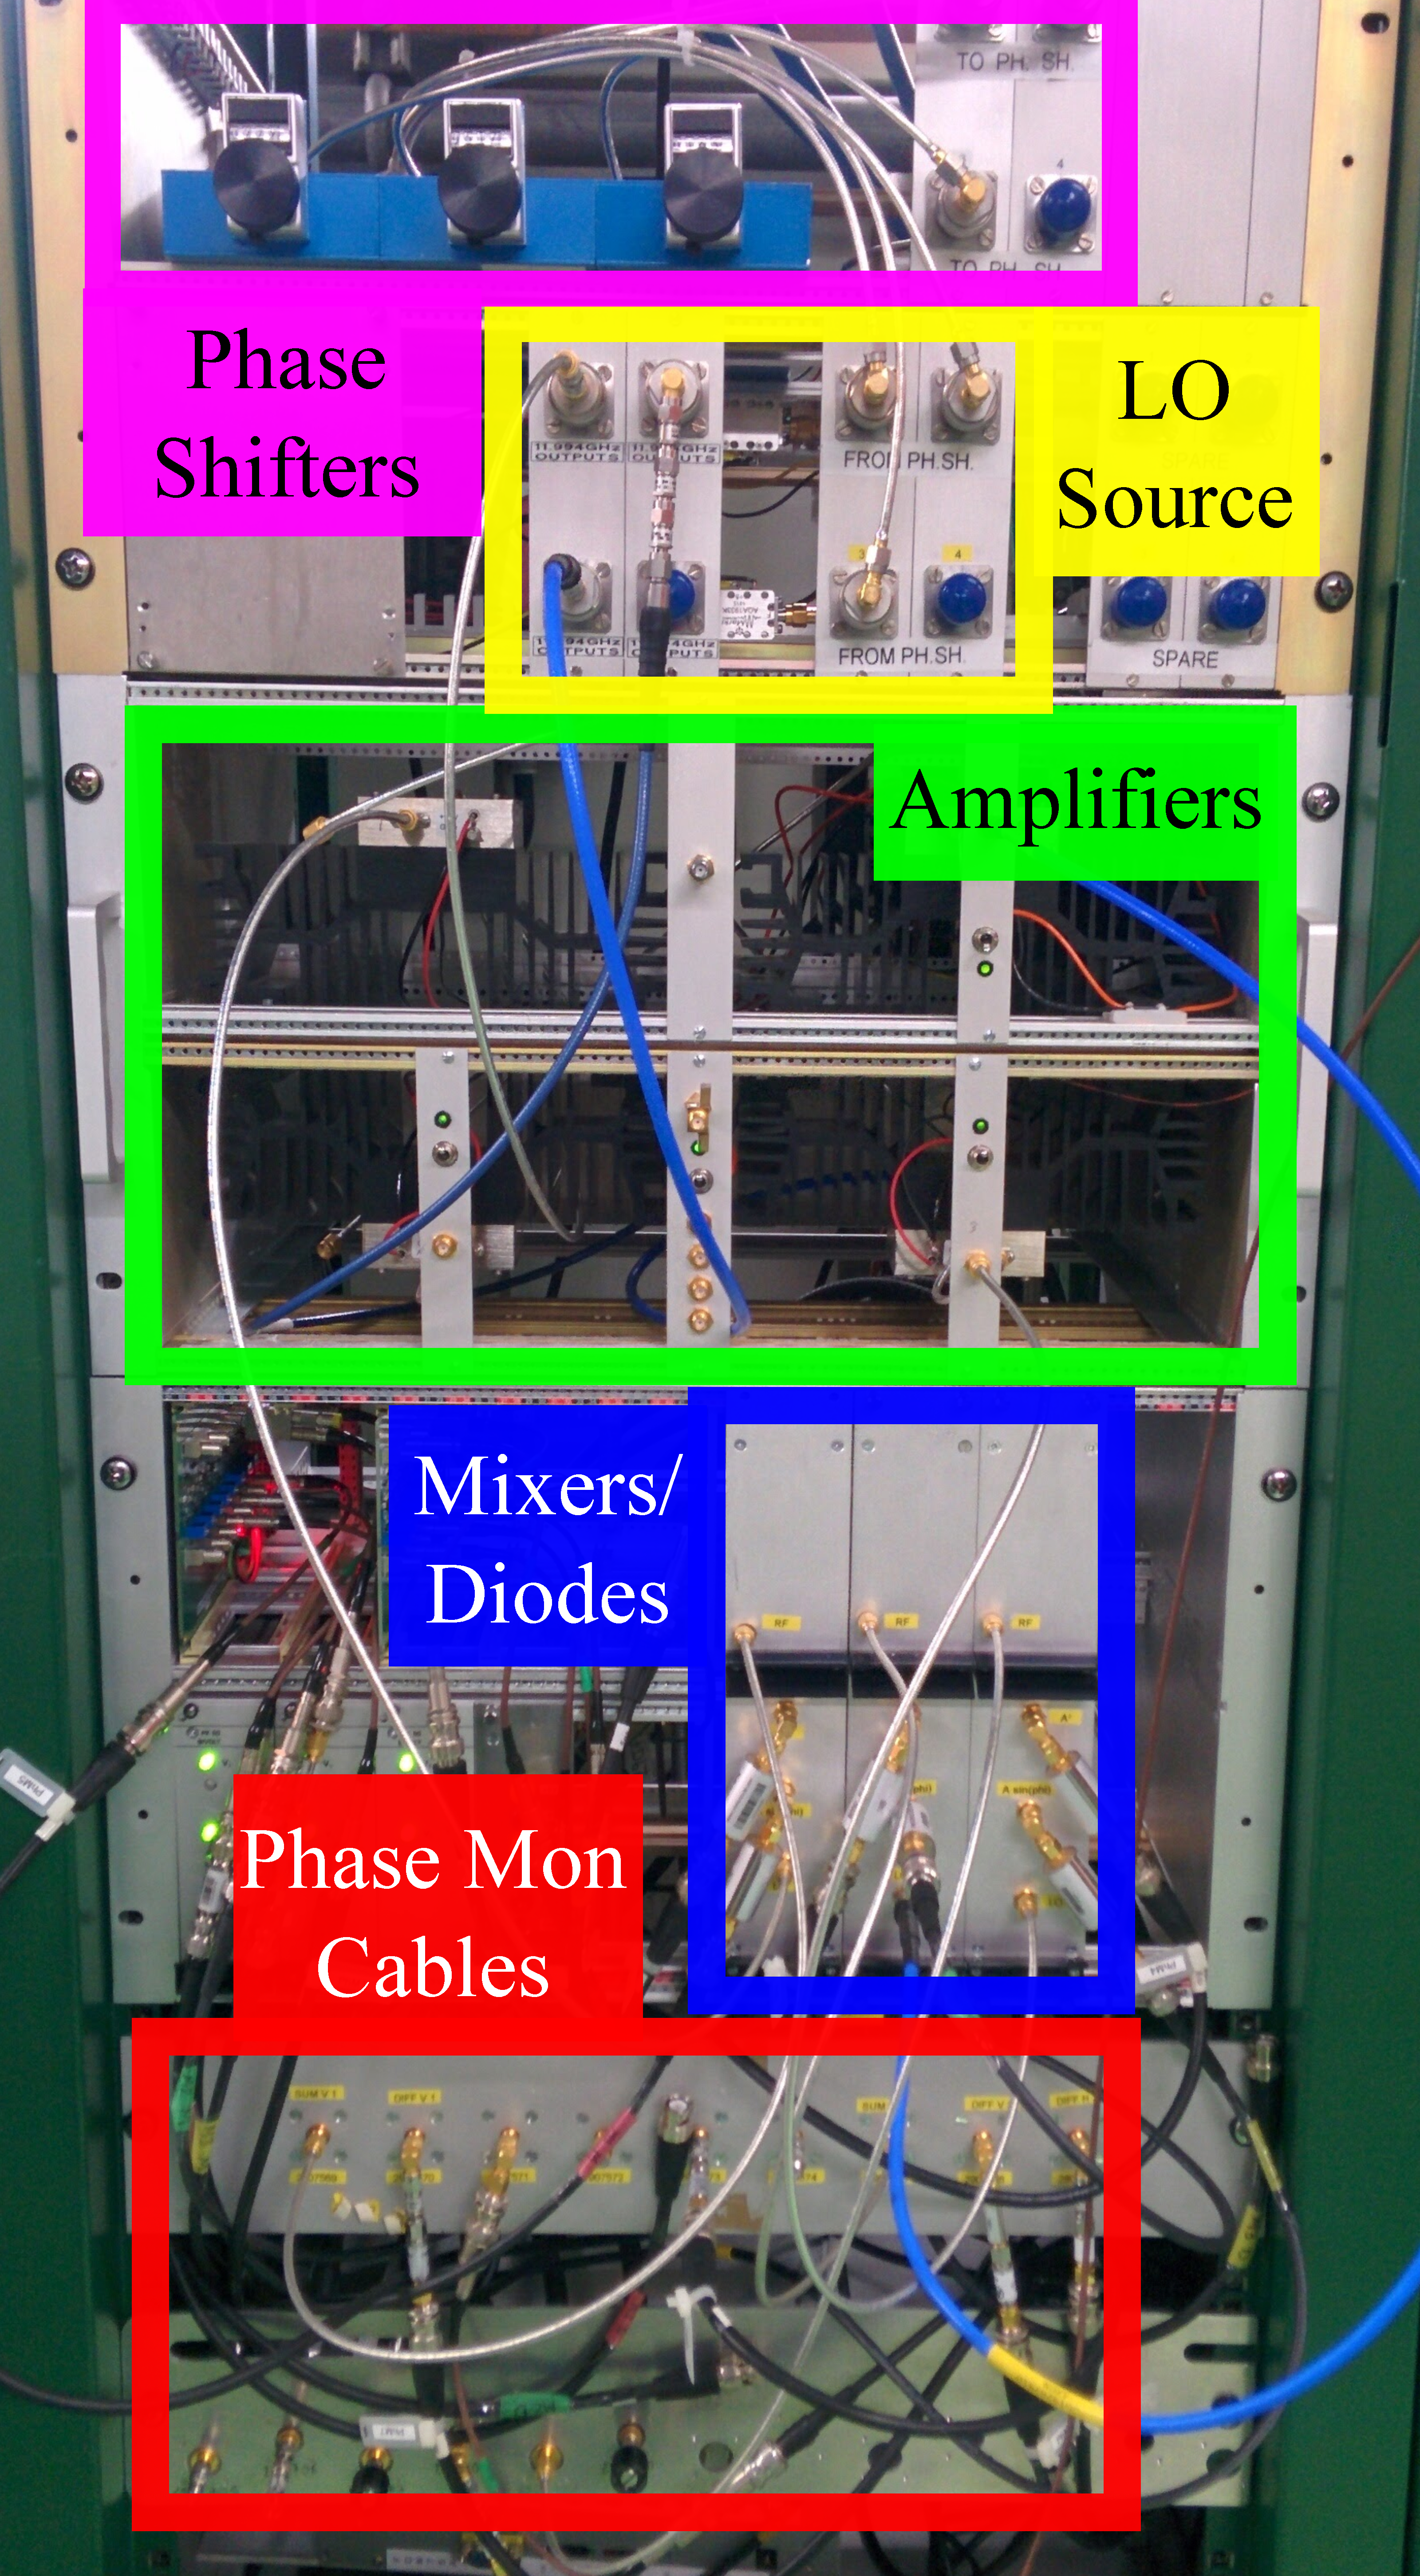
\includegraphics[width=\columnwidth]{phMonRack}% Here is 
%  %how to 
%  %import EPS art
%  \caption{\label{f:phMonRack}
%  }
%\end{figure}


\begin{figure}
  \centering
  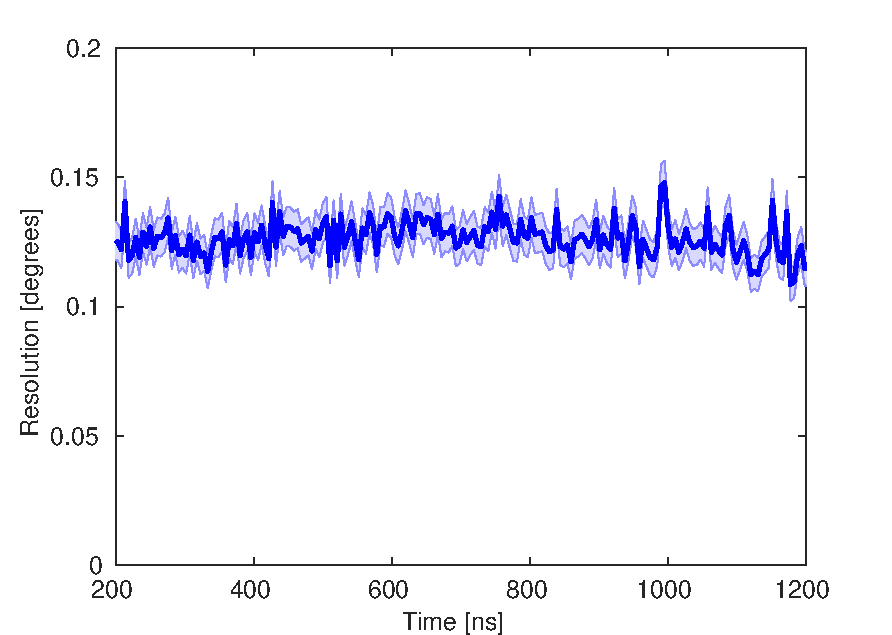
\includegraphics[width=0.66\columnwidth]{phMonRes}% Here is 
  %how to 
  %import EPS art
  \caption{\label{f:phMonRes}
  }
\end{figure}

%\begin{figure}
%  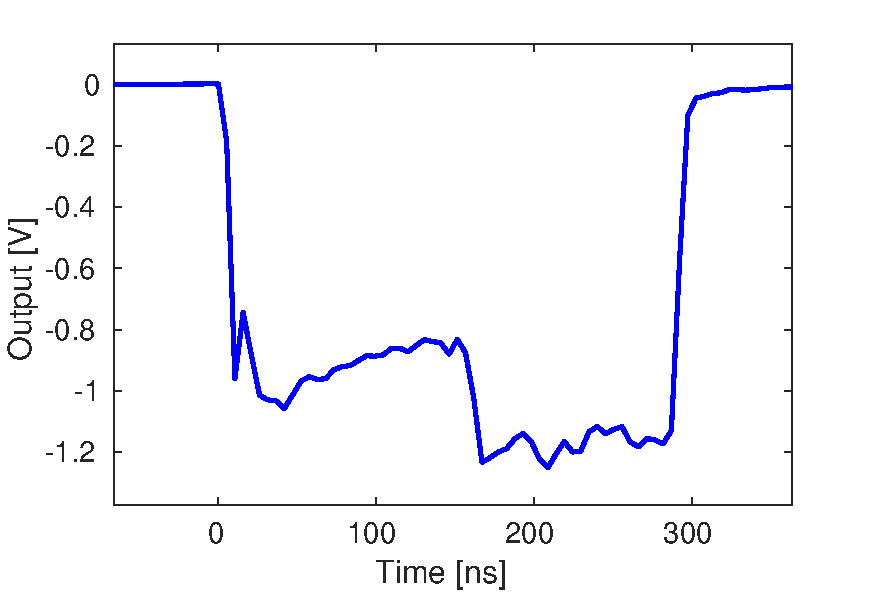
\includegraphics[width=\columnwidth]{phMonBw}
%  \caption{\label{f:phMonBw}
%  }
%\end{figure}

\begin{figure}
  \centering
  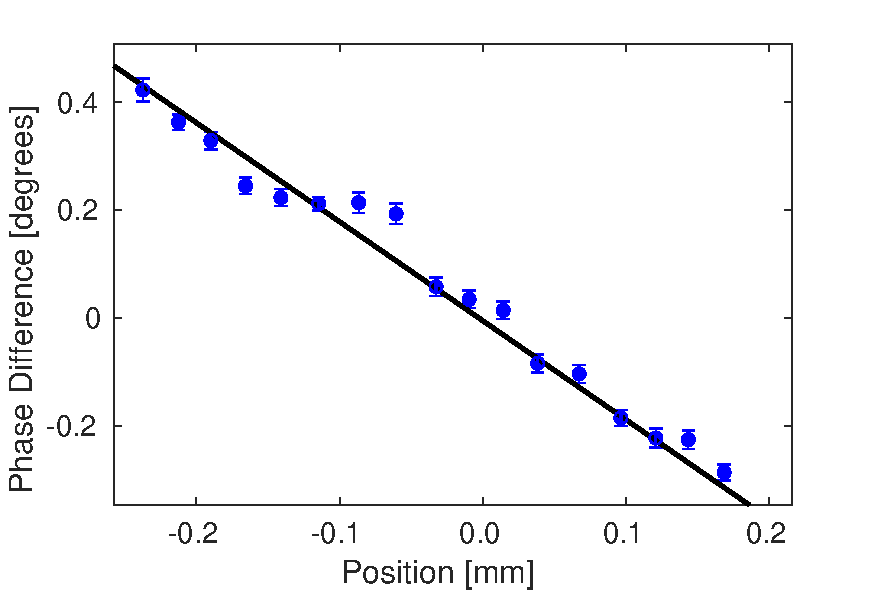
\includegraphics[width=0.66\columnwidth]{phMonHScan}% Here is 
  %how to 
  %import EPS art
  \caption{\label{f:phMonHScan}
  }
\end{figure}

\subsection{\label{ss:font}Feedforward Controller}

% FROM THESIS
The basic logic of the firmware is as follows. The ADC sampling and timing are 
defined by the input trigger and external 357~MHz clock. The ADC outputs are 
processed continuously on the FPGA, including the addition of channel offsets 
and the application of filters. Then the processed ADC~2 (Mixer) output is 
split in two, creating the two parallel strands that become the DAC~1 and DAC~2 
outputs. Note that, instead of using arcsine, the Mixer value is used directly 
in the calculation, thereby assuming the small angle approximation. 
Prior to being sent to the DACs the two output strands are 
multiplied by their corresponding gain factors, as set in the DAQ. An 
additional delay can be added to the DAC outputs, allowing the synchronisation 
of the correction with the beam to be adjusted. The two calculated DAC outputs 
are connected to the amplifier drive inputs, where they are amplified and 
eventually output to the kickers to deflect the beam and correct the phase. 
The overall latency of the FONT5a board, from the arrival of the signal at the 
ADCs to the output of the calculated correction at the DACs, is around 22 clock 
cycles (at 357~MHz) or 60~ns \cite{glennCLIC14}.
% /FROM THESIS

%\begin{figure}
%  \includegraphics[width=\columnwidth]{FONT5aPanel}% Here is 
%  %how to 
%  %import EPS art
%  \caption{\label{f:FONT5aPanel}
%  }
%\end{figure}

\begin{figure}
  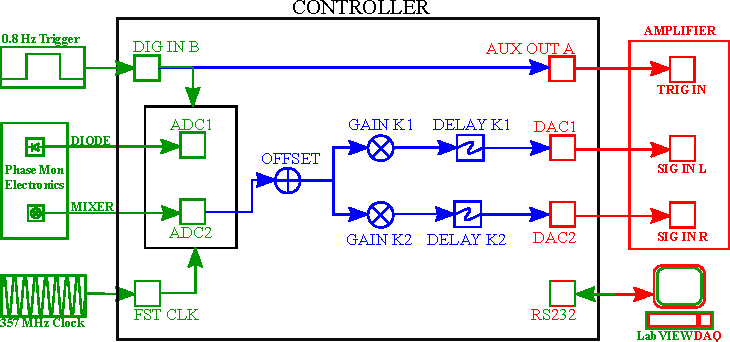
\includegraphics[width=\columnwidth]{fontDiagram}% Here is 
  %how to 
  %import EPS art
  \caption{\label{f:fontDiagram}
  }
\end{figure}

% FROM THESIS
In the PFF system the voltage sent to the kickers in the TL2 chicane (see 
Figures~\ref{f:ctfpffLayout}~and~\ref{f:newTL2Lattice}) is varied depending on 
the upstream phase. The corrected downstream phase, \(\phi_{PFF}\), can 
therefore be simply modelled as subtracting the upstream phase, \(\phi_u\), 
from the initial downstream phase \(\phi_d\):
\begin{equation}
\phi_{PFF} = \phi_d - g\phi_u
\label{e:pffEq1}
\end{equation}
\begin{equation}
g = \rho_{ud}\left(\frac{\sigma_d}{\sigma_u}\right)
\label{e:theoretOptGain}
\end{equation}
\begin{equation}
\sigma_{PFF} = \sigma_d\sqrt{1-\rho_{ud}^2}
\end{equation}
%/FROM THESIS


\subsection{\label{ss:amp}Amplifiers}

% FROM THESIS
The amplifier takes the two DAC signals from the FONT5a board and
uses them to produce four high voltage outputs. These are connected to the 
downstream ends of the kicker strips (two kickers and two strips per kicker 
gives four connections at the downstream ends in total), creating the potential 
difference between the strips that deflects the beam in order to correct the 
phase. The returning signals from the upstream ends of the kicker strips are 
then terminated back at the amplifier.

\begin{figure}
  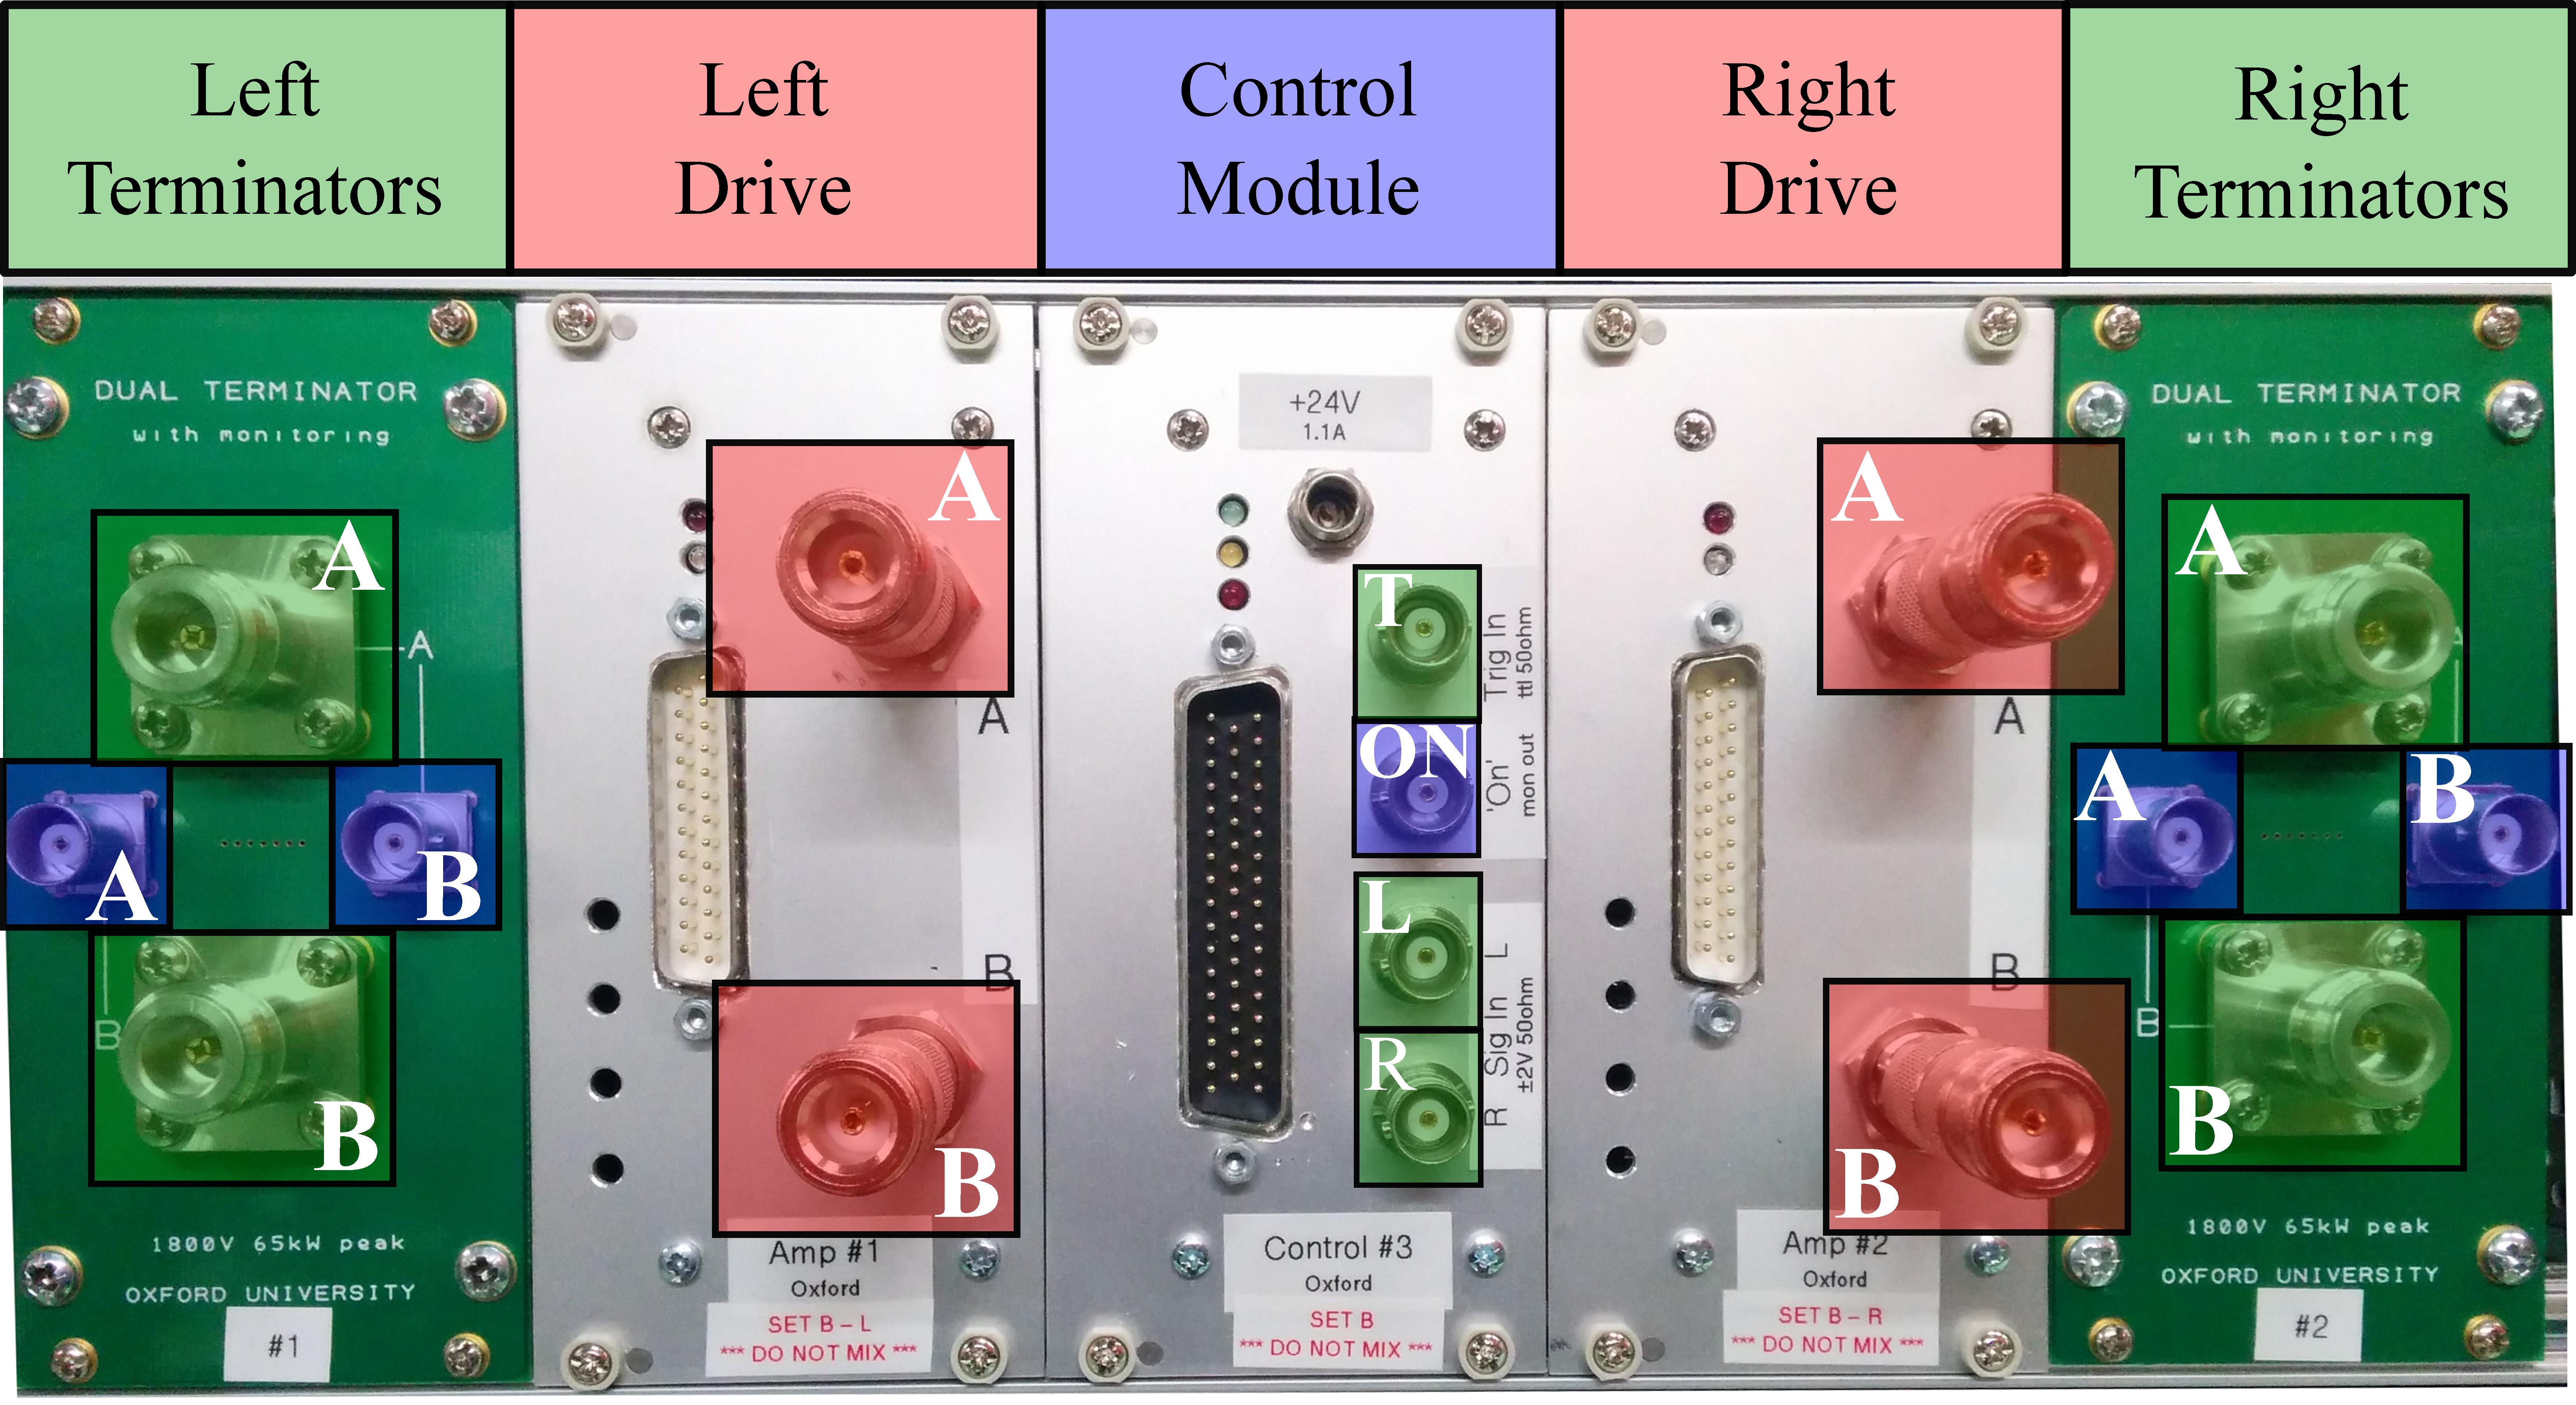
\includegraphics[width=\columnwidth]{AmpPanel}% Here is 
  %how to 
  %import EPS art
  \caption{\label{f:AmpPanel}
  }
\end{figure}

The amplifier is purpose built for the PFF prototype, also at Oxford 
University, with further details of its design available in \cite{colinCLIC16}. 
An annotated picture of its front panel is shown in 
Figure~\ref{f:AmplifierPanelPic} and a simplified diagram showing the flow of 
signals between the FONT5a board, amplifier and kickers is shown in 
Figure~\ref{f:amplifierDiagram}.
The amplifier is installed in a standard 3U rack and has a modular design. It 
consists of five individual modules split between two sides, labelled left and 
right. The left side of the amplifier, which uses the DAC~1 output, powers the 
first kicker in the chicane, and the right side of the amplifier, which uses 
the DAC~2 output, powers the second kicker. Each side of the amplifier contains 
its own ``drive module'' and ``terminator module''. Finally there is a central 
``control module'' that is common to both sides of the amplifier.

\begin{figure}
  \subfloat[]
   {
    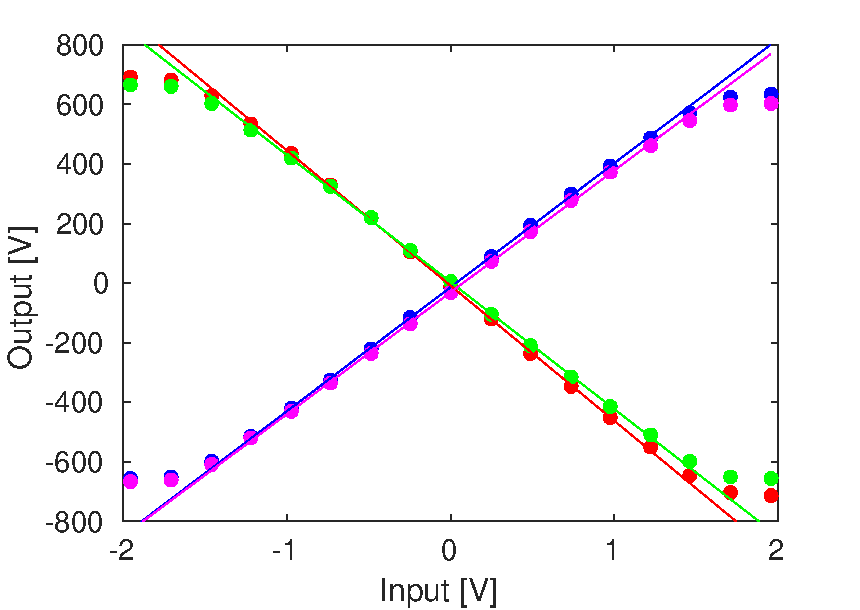
\includegraphics[width=0.5\textwidth]{AmpOutvsDAC}
    \label{f:AmpOutvsDAC}
   } 
  \hfill
  \subfloat[]
   {
    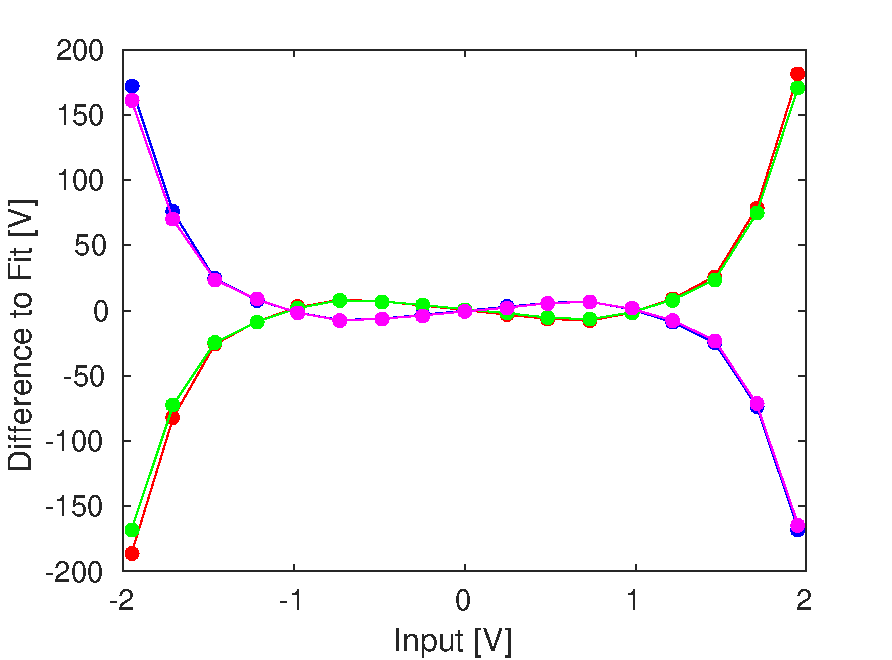
\includegraphics[width=0.5\textwidth]{AmpOutvsDAC_residual}
    \label{f:AmpOutvsDAC_residual}
   } 
  \caption{\label{f:AmpOutvsDACFig}test \ref{f:AmpOutvsDAC}}
\end{figure}

Figure~\ref{f:AmpOutvsDAC} shows the amplifier output, measured using the 
monitoring signals, at different constant input voltages sent from the FONT5a 
board between the minimum of -2V (-4095 DAC counts) and maximum of 2V (+4095 
DAC counts). The amplitude of the monitoring signals is converted in to the 
amplifier output voltage using the approximate conversion factor of 115 
\cite{colinPriv}. All four amplifier outputs are shown (one for each strip of 
the two kickers). The values plotted are the mean of the 480~ns central region 
of the whole 1400~ns output pulse.

The response of the amplifier is linear up to \(\pm1.2\)~V input voltage. 
Outside this range the amplifier clearly begins to enter saturation, in 
particular above input voltages of \(\pm1.7\)~V. The linear fits shown include 
only the points up to \(\pm1.2\)~V, in order to not be biased by the effects of 
saturation. Figure \ref{f:AmpOutvsDAC_residual} shows the difference between 
the linear fit and the measured amplifier output across the full range of input 
voltages. A slight deviation from linearity in the \(\pm1.2\)~V range is also 
visible, although the maximum difference is only 10~V or a 3\% relative error.

Figures~\ref{f:ampLTraces} and \ref{f:ampRTraces} show the full 
1.4~\(\mathrm{\mu}\)s amplifier output with a constant input of \(+1\)~V 
(\(-1\)~V) applied to the left (right) amplifier respectively. Spikes in the 
signal just prior to 2000~ns and after 3000~ns on the time axis as seen in the 
plots are pickup on the kicker strips induced by the beam. For a constant input 
voltage the output voltage along the pulse varies by up to 88~V peak-to-peak 
(mean 12~V) for the left amplifier or 93~V peak-to-peak (mean 14~V) for the 
right amplifier. As a relative difference, this corresponds to approximately a 
6~\% peak-to-peak, or 1~\% mean, variation along the pulse.
% / FROM THESIS

Brief design

Linearity

Pulse shape

\begin{figure}
 \centering
  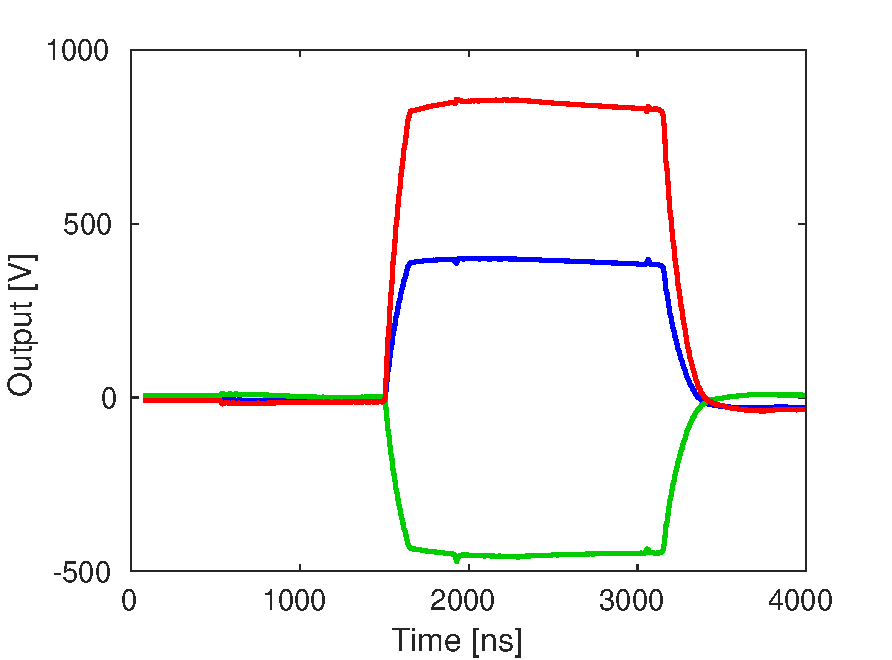
\includegraphics[width=0.66\columnwidth]{AmpL_Traces}% Here is 
  %how to 
  %import EPS art
  \caption{\label{f:AmpL_Traces} AmpL Traces
  }
\end{figure}

\subsection{\label{ss:kick}Kickers}

% FROM THESIS
The two electromagnetic kickers provide the phase correction in the PFF system 
by deflecting the beam on to longer or shorter paths in the TL2 chicane (see 
Figure~\ref{f:ctfpffLayout}). They have been designed and built by INFN, Italy 
\cite{infn}, based on a similar design used at the DA\(\mathrm{\Phi}\)NE 
collider \cite{dafneKick}. A schematic of the kicker design is shown in 
Figure~\ref{f:kickerSchematic}. It consists of two parallel conducting strips 
placed along the left and right side of the beam pipe. Each strip is 
approximately one metre in length and the horizontal separation between the 
strips is 40~mm. The strips are tapered at their ends to reduce coupling 
impedance (to reduce the voltage induced on the strips by the beam) 
\cite{kickerIPAC11}.
% /FROM THESIS

Brief design, cable connections etc.

\begin{figure}
  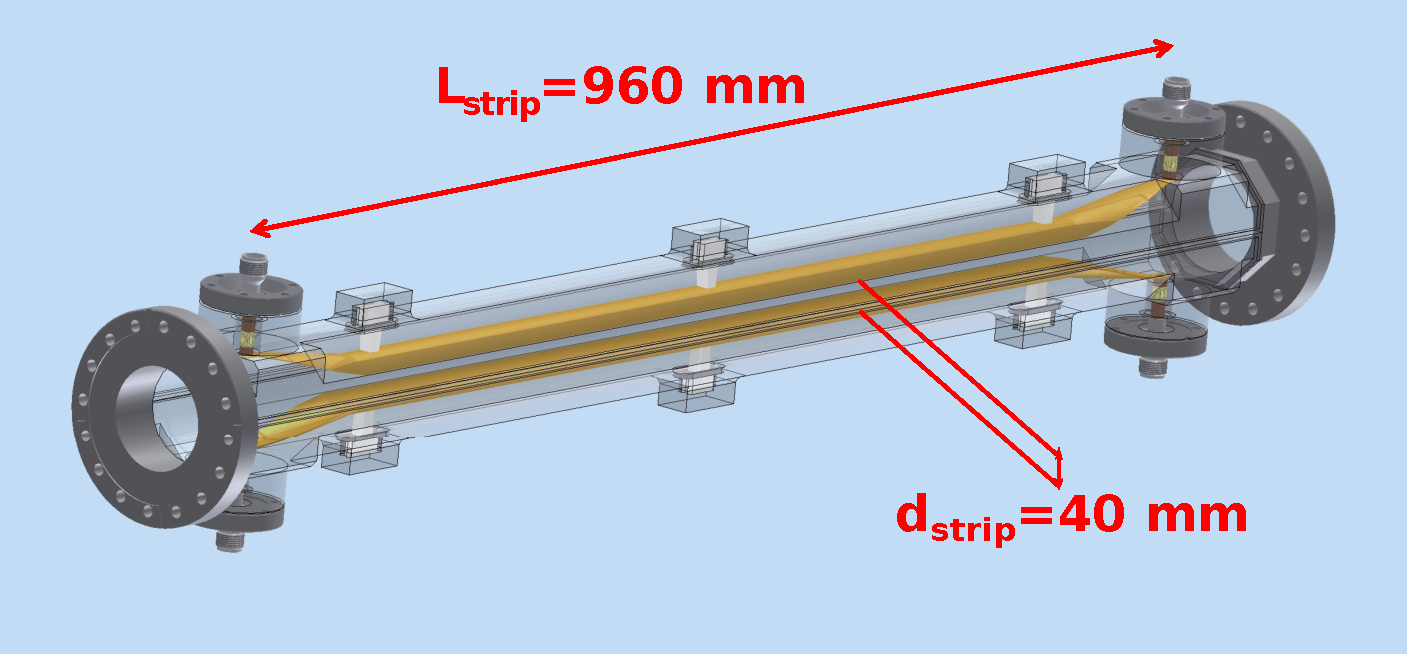
\includegraphics[width=\columnwidth]{kickerSchematic}% Here is 
  %how to 
  %import EPS art
  \caption{\label{f:kickerSchematic}
  }
\end{figure}

